% !BIB TS-program = biber
\documentclass{frontiersSCNS} % for Science articles



\usepackage{graphicx}
%
\usepackage{amsmath} 
\usepackage{mathptmx}      % use Times fonts if available on your TeX system
%
\usepackage{color, soul}

\usepackage{caption}
\usepackage{float}
\floatstyle{plaintop}

\usepackage{hyperref}

% bibliography
\usepackage[english]{babel}
\usepackage{csquotes}
\usepackage[
backend=biber, 
bibencoding=utf8, 
style=authoryear, 
date=year, 
maxbibnames=6, 
minbibnames=6, 
url=false, 
isbn=false, 
eprint=false,
uniquename = false, 
autocite=inline]{biblatex}
\addbibresource{Bibliography.bib}

\usepackage[draft, nomargin, marginclue, footnote]{fixme}
\fxsetup{targetlayout=color}

% new commands and shortcuts
\usepackage{xspace}
\newcommand{\eg}{\textit{e.g.}\xspace}
\newcommand{\etal}{\textit{et al.}\xspace}
\newcommand{\ie}{\textit{i.e.}\xspace}
\newcommand{\etc}{\textit{etc.}\xspace}
\newcommand{\vs}{\textit{vs.}\xspace}
\newcommand{\viz}{\textit{viz.}\xspace}

% shortcut for float placing
\usepackage{placeins}

% make pretty MATLAB code
\usepackage{listings}
\usepackage{matlab-prettifier}
\lstMakeShortInline[style=Matlab-editor]"

% other nice features
\usepackage{lineno}
\linenumbers

\usepackage{xifthen}% provides \isempty test

\copyrightyear{}
\pubyear{}

\def\journal{Neuroinformatics}
\def\DOI{}
\def\articleType{Technology Report}
\def\keyFont{\fontsize{8}{11}\helveticabold }
\def\firstAuthorLast{Gorur-Shandilya, Hoyland \& Marder} 
\def\Authors{Srinivas Gorur-Shandilya\,$^{1*\dagger}$, Alec Hoyland\,$^{1\dagger}$, and Eve Marder$^{1}$}
\def\Address{$^{1}$Volen National Center for Complex Systems and Biology Department \\ Brandeis University \\ Waltham, MA 02453 \\ USA
\vspace{0.25cm}

\vspace{0.5em}\tiny{$\dagger$ These authors have equally contributed to this article.}
}
\def\corrAuthor{Srinivas Gorur-Shandilya }
%\def\corrAddress{Marder Lab, Brandeis University, Biology Department and Volen Center for Complex Systems, Waltham, MA, USA}
\def\corrAddress{Volen National Center for Complex Systems, Brandeis University, Waltham MA 02453}
\def\corrEmail{\texttt{srinivasgs@brandeis.edu}}

\newcommand{\dd}[1]{\mathrm{d}#1}

\begin{document}
\onecolumn
\firstpage{1}

\title[xolotl: neuron \& network simulator]{Xolotl: An Intuitive and Approachable Neuron \& Network Simulator in MATLAB}
\author[\firstAuthorLast ]{\Authors}
\address{}
\correspondance{}
\extraAuth{}
\topic{An Intuitive Neuronal Simulator}

\maketitle

\begin{abstract}
	

	Conductance-based models of neurons have been used extensively in computational neuroscience. However, working with these models continues to be a challenge due to their high dimensionality and large number of parameters, that hinders intuition of their dynamical features. Here, we present a neuron and network simulator built on a novel automatic type system that binds class templates written in "C++" to object-oriented code in "MATLAB". Our approach builds on the tradition of uniting the speed and power of languages like "C++" with the ease-of-use and feature-set of scientific programming languages like "MATLAB". Our software allows for the creation and manipulation of hierarchical models with components that are named and searchable, permitting intuitive high-level programmatic control over all parameters. Our simulator's architecture allows for the live manipulation of any parameter in any model, and for visualizing the effects of changing that parameter immediately. Our simulator is fully featured with hundreds of ion channel models from the electrophysiological literature, and can be extended to include arbitrary conductances, synapses, and mechanisms. Finally, our simulator is written in a modular fashion and has been released under a permissive free software license, enabling seamless integration into the workflow of many researchers.
	
	\tiny
	\keyFont{ \section{Keywords:} simulator, code:MATLAB, code:C++, conductance-based, neuron, network, pedagogy}
	
\end{abstract}

%%%%%%%%%%%%%%%%%%%%%%%%%%%%%%%%%
%  								%
%		INTRODUCTION 			%
% 		& OVERVIEW   			%
%								%
%								%
%%%%%%%%%%%%%%%%%%%%%%%%%%%%%%%%%

\section{Introduction}
\label{sec:intro}

Nervous systems process and transmit information using electrically excitable membranes. Conductance-based models are a powerful biophysical simplification of an electrically excitable compartment in a neuron (\cite{hodgkinQuantitativeDescriptionMembrane1952a}). Studies based on the Hodgkin-Huxley formalism now contribute significantly to mainstream research in small circuits (\cite{marderTheoryMotion1995, prinzComputationalApproachesNeuronal2010, prinzInsightsModelsRhythmic2006}). These models provide an approachable framework for understanding many salient principles of neuroscience, since they explicitly model cell membranes and ion channels as electrical components in a circuit. However, several challenges remain in working with biophysically-detailed conductance-based neuron models. First, these models can be high-dimensional with many nonlinear differential equations, each with several parameters. Second, many or all equations in these models can be strongly coupled through dynamic variables like the membrane potential.  In multi-compartment models of spatially extended neurons, membrane potentials in every compartment can be different, and are coupled to each other. Finally, the choice of programming language used to implement the model imposes tradeoffs in designing and using neuron and network simulators: simulators written in languages like "C++" or "FORTRAN" can integrate equations quickly, but often lack the ease-of-use and interoperability of those written in scientific programming languages like "Python", "Julia" or "MATLAB". 

Two major approaches have dominated the design of neuron simulators. First, some simulators, such as "NEURON" (\cite{hinesNEURONSimulationEnvironment1997}) are written in a fast compiled language like "C" and allow for the construction and simulation of neuron models using object-oriented paradigms. These simulators tend to perform fast computations with little overhead, but suffer from a steep learning curve. Wrapping these simulators in a more approachable language like "Python" and the use of graphical user interfaces (GUIs) mitigate these drawbacks (\cite{hinesNEURONPython2009}), at the cost of obfuscating the underlying algorithms and parameters (\cite{bretteSimulationNetworksSpiking2007, hinesNEURONPython2009}). Another approach is to design simulators that can be used entirely in popular scientific programming languages. These simulators can be easier to use, and can benefit from inter-compatibility with other tools. Programs like "DynaSim" (\cite{sherfeyDynaSimMATLABToolbox2018}), "ANNarchy" (\cite{vitayANNarchyCodeGeneration2015}), "BRIAN" (\cite{stimbergBrianSecondComing2013}), "morphforge" (\cite{hullMorphforgeToolboxSimulating2014}), "PyNN" (\cite{davisonPyNNCommonInterface2009}) allow the user to specify models with strings of equations or with components that are constructed using a special syntax, that can then be translated into a faster implementation language such as "C" or "C++" (\cite{stimbergEquationorientedSpecificationNeural2014}). This approach permits considerable flexibility for simulating systems of differential equations. Since models need to be translated between the two languages, the hierarchical nature of neuron models is not naturally encapsulated by these tools, and the syntax can be verbose. Neither approach facilitates the creation of tools that simultaneously maintain efficiency, ease-of-use, and clarity.

To overcome these design limitations, we have developed a novel automatic type system, "cpplab", which binds "MATLAB" code to "C++" header files. This architecture automatically creates objects in "MATLAB" that represent the underlying object-oriented "C++" code, without having to re-specify these objects in "MATLAB". In this paper, we introduce "xolotl", an implementation of the "cpplab" system specialized in integrating conductance-based neuron and network models. Models can be easily constructed from network building blocks in a few lines of "MATLAB" code using a hierarchical and intuitive syntax. Since models in the "MATLAB" workspace are automatically linked to models in the "C++" implementation, configuring these objects in "MATLAB" transparently configures the underlying "C++" objects. "xolotl" comes packaged with hundreds of components that can be used to assemble cells and networks;  has built-in visualization functions to inspect voltage time traces and activation functions; and a GUI for real-time manipulation of model parameters. The ease-of-use of the tools built into our software lends them to pedagogical applications and the rapid prototyping of models. Our software aims to simplify the investigation of the dynamics of conductance-based network and neuron models, facilitate collaborative modeling, and is intended to complement other tools being developed in the computational neuroscience community.


%%%%%%%%%%%%%%%%%%%%%%%%%%%%%%%%%%%%%%%%%%%%%%%%%%%%%%%%%%%%%%
%
%
%
%		DESIGN GOALS
%
%
%
%%%%%%%%%%%%%%%%%%%%%%%%%%%%%%%%%%%%%%%%%%%%%%%%%%%%%%%%%

\section{Design Goals}
\label{design}

"xolotl" is designed to be easy-to-use and richly featured while being fast enough to use in everyday research. Our focus was on designing an approachable simulator of conductance-based neurons and networks of these neurons; simulating arbitrary dynamical systems is therefore beyond the scope of this software. Specifically, the software was designed to simulate models of the form 


\begin{equation}
C_{i}\frac{dV_{i}}{dt}=-\sum_{j}I_{j} \label{eq:1}
\end{equation}

where \( C_{i} \) and  \( V_{i} \) are the capacitance and membrane potential of compartment  \( i \) and \( I_{j} \) is the current due to ion channel population \( j \) given by 

\begin{equation}
I_{j}=\bar{g}_{j}m_{j}^{p}h_{j}^{q}(V-E_{j})A_{i}  \label{eq:2}
\end{equation}

Here, \( \bar{g}_{j} \) is the maximal conductance, and \( E_{j} \) is the reversal potential of the ion channel population \( j \). \( A_{i} \) is the surface area of compartment \( i\) that contains these ion channels.  \( m_{j} \) and \( h_{j} \) are activation and inactivation variables that change according to

\begin{eqnarray*}
\tau_{m}\frac{dm}{dt}=m_{\infty}-m & \mathrm{and} & \tau_{h}\frac{dh}{dt}=h_{\infty}-h
\end{eqnarray*}

Typically, \( \tau_{m} \), \( \tau_{h} \), \( m_{\infty} \), and \( h_{\infty} \) are functions of the membrane potential \( V_{i} \). The software uses integration schemes that have been specifically developed to solve equations of this form (\cite{dayanTheoreticalNeuroscience2001, hinesEfficientComputationBranched1984, ohErrorAnalysisSpecialized2006}), though other schemes can be used if desired.   

This software is designed to be used from within "MATLAB", a scientific programming language common amongst neuroscientists and engineers for pedagogy and research. Our goal was to make "xolotl" completely usable entirely from within MATLAB, and fully scriptable. Models created using this simulator appear in the "MATLAB" workspace as native objects, and are thus fully compatible with the large library of toolboxes that "MATLAB" provides, allowing so the software to be used as a component of other packages and tools. All parameters of models and activation functions of any channel can be be inspected before running the model. We designed several features of the simulator to be easily extensible: adding custom conductances or synapse types is possible by calling functions that generate new "C++" files on the fly. Finally, "xolotl" is designed to be fully auditable, and comes with several tools to verify model and parameter integrity and aid reproducibility. 



\subsection{Features}
\label{features}

\paragraph{A rich library of network components.} "xolotl" comes packaged with hundreds of pre-existing components (compartments, synapses, conductances, and mechanisms) that can be used as building blocks to construct model neurons and networks. Compartments represent sections of membrane with a single membrane potential, Calcium level, and set of constituent components; and can represent either entire cells or parts of cells. Objects of type "conductance" represent populations of ion channels in a compartment that produce transmembrane currents. Objects of type "synapse" connect two compartments together by introducing a current in the post-synaptic neuron that can depend on the voltage of the presynaptic neuron. Objects of type "mechanism" can represent any intracellular mechanism and can read and modify any other component in the cell, and can run arbitrary dynamical systems within them. 

\paragraph{Object-oriented.}
"xolotl" is designed to mirror the nested and hierarchical structure of networks and neurons. Biological neuronal networks are made up of neurons that are connected to each other with synapses. Each of these neurons contains within it a set of conductances and synaptic currents that contribute to its electrical behavior. Intracellular mechanisms can act within the cell to modify and regulate conductances, synapses, or the dynamic properties of the cell. Similarly, a "xolotl" model can contain a set of compartments that can represent individual neurons. Each compartment can contain a arbitrary set of conductances, and compartments, conductances and synapses can contain mechanisms that affect anything in the model. All objects in the "xolotl" model tree (compartments, conductances, etc.) are bonafide "MATLAB" objects that have their own type, properties and associated methods. This object-oriented programming paradigm naturally represents the hierarchical structure of biological networks that contain neurons that contain populations of ion channels, and makes constructing, integrating and thinking about these models easier. 

\paragraph{Automatic type system.}
Our approach to circumvent the tradeoff between high-performance but hard to use languages like "C++" and richly featured but potentially slow languages like "MATLAB" was to construct an automatic type system that links object oriented code in "C++" to object oriented code in "MATLAB". This architecture lets us construct the core of the simulator in "C++", leveraging features of "C++" like pointers that are not readily available in "MATLAB". A rudimentary way to make this "C++" code useable in "MATLAB" would be to re-write that code in "MATLAB" so that "MATLAB" objects can be bound their "C++" implementations. However, this approach is cumbersome, and prone to errors, since the same code needs to be written twice, in two languages. Instead, our automatic type system creates objects in "MATLAB" on-the-fly  from "C++" class specifications, obviating the need to rewrite code in "MATLAB" while preserving a tight coupling between objects in the "MATLAB" workspace and their "C++" implementation. The key advantages of this approach are that it makes developing new code much easier, and simplifies the task of constructing complex frameworks that span these two languages. 

\paragraph{Automatic hashing and compiling.}
Since every model requires a compiled binary to run, a potential stumbling block is the problem of unambiguously linking a model to a binary executable. "xolotl" solves this problem by hashing the "C++" header files of every component in the model recursively, allowing a model, no matter how complex, to be compactly represented by a short alphanumeric identifier (its "hash"). Compiled binaries are named using this hash, ensuring both that the correct binary is run to integrate the model, and that compilation occurs only as needed. This powerful feature enables the user experience to remain entirely within the "MATLAB" workspace, with compilation and selection of the correct binary occurring silently in the background. 


\subsection{Limitations}
\label{limitations}

Our focus on ease-of-use and speed means some features were intentionally neglected in the design process. 

\paragraph{Limited to conductance-based models.} "xolotl" has been developed specifically for conductance-based models. It does not currently support rate- or current-based models, or arbitrary dynamical systems. 

\paragraph{Limited numerical integration strategies.} Most components in the software are integrated using the exponential Euler method, which has been shown to perform well in neuronal models (\cite{ohErrorAnalysisSpecialized2006, dayanTheoreticalNeuroscience2001}. However, it may be desirable to use other methods under certain conditions. It is possible to introduce new network components that implement other integration schemes, or to modify the integration schemes of existing components, but that requires writing new "C++"  code, and is still restricted to integration schemes that assume a fixed step size. 

\paragraph{Inefficient tools for handling large networks.} "xolotl" was designed to work with small but complex networks and models, where every compartment and component is $named$, rather than numbered. It is more therefore suited towards simulating small and heterogeneous networks rather than large but homogenous networks. While the software $can$ integrate large networks ($>1000$ compartments), other tools are presumably more suited to this task, offer more natural frameworks for dealing with a large number of identical units.  

\paragraph{New mechanisms require new \texttt{C++} code.} Adding new network components requires writing new "C++" code. Adding a new conductance in the Hodgkin-Huxley formalism (\cite{hodgkinComponentsMembraneConductance1952, hodgkinMeasurementCurrentvoltageRelations1952a, hodgkinQuantitativeDescriptionMembrane1952a, dayanTheoreticalNeuroscience2001}), requires creating a new "C++" header file, though this is generally trivial. Implementing a new integration scheme or component type requires much more in-depth knowledge of the underlying "C++" core code.

%%%%%%%%%%%%%%%%%%%%%%%%%%%%%%%%%%%%%%%%%%%%%%%%%%%%%%%%%%%%%%%%%%
%
%
%
%		USAGE EXAMPLES
%
%
%
%%%%%%%%%%%%%%%%%%%%%%%%%%%%%%%%%%%%%%%%%%%%%%%%%%%%%%%%%%%%%%%%%%

\section{Usage Examples}
\label{usage}

In this section, we illustrate how "xolotl" can be used to generate a variety of models and simulate them. These examples have been chosen to illustrate various features of "xolotl", and are intended to serve as templates that researchers and educators can build upon.

%%%%%%%%%%%%%%%%%%%%%%%%%%%%%%%%%%%%%%%%%%%%%%%%%%%%%%%%%%%%%%%%%%
%
%
%
%		SIMULATING A HODGKIN-HUXLEY MODEL
%
%
%
%%%%%%%%%%%%%%%%%%%%%%%%%%%%%%%%%%%%%%%%%%%%%%%%%%%%%%%%%%%%%%%%%%

\subsection{Simulating a Hodgkin-Huxley Model}

The axon of the giant squid contains contains a fast inactivating sodium conductance ("NaV"), a slower non-inactivating potassium conductance ("Kd"), and a passive leak current ("Leak"). Seminal work by Hodgkin and Huxley showed that depolarizations of the membrane, for example, by injecting current, could lead to an activation of the voltage-sensitive "NaV" channels, which led to a run away depolarization that was terminated by the inactivation of "NaV" channels and the activation of "Kd" channels that repolarized the membrane (\cite{hodgkinComponentsMembraneConductance1952, hodgkinMeasurementCurrentvoltageRelations1952a}). As one of the simplest models of excitable neural membranes, the Hodgkin-Huxley model often serves as a the first model introduced in pedagogical literature (\cite{dayanTheoreticalNeuroscience2001, sterrattPrinciplesComputationalModelling2011, trappenbergFundamentalsComputationalNeuroscience2010}).  


In this example, we demonstrate how to simulate the spiking activity of a Hodgkin-Huxley-like model, and how the tools built into our simulator make it easy to set up and integrate the model, and gain insight into the underlying biophysical mechanism. This simple model consists of a single-compartment neuron with three types of conductances  (Figure \ref{fig:figurehh}A). This hierarchical organization of the neuron is mirrored in the structure of the model: an object of type "compartment" is used to represent the cell body, and three objects of type "conductance" are used to model the three populations of ion channels (Figure \ref{fig:figurehh}B). These models of ion channels were obtained from \cite{liuModelNeuronActivityDependent1998} based on electrophysiological recordings from the lobster stomatogastric ganglion (\cite{turrigianoSelectiveRegulationCurrent1995}), and are part of the simulator. The syntax of constructing the neuron model (using "add" statements) preserves this hierarchical organization, and the code snippet in (Figure \ref{fig:figurehh}C) shows how this model can be created using just a few lines of code. 

Adding an injected current and calling the built-in "plot" function plots the time series of membrane voltage. In the absence of injected current, the model is quiescent. When 0.2 nA is injected, the model tonically spikes (Figure \ref{fig:figurehh}A-B).  The \texttt{plot} function displays a voltage trace colored by the dominant current (Figure \ref{fig:figurehh}A). Colors in the voltage trace indicate the strongest instantaneous inward current when the voltage is increasing, and strongest instantaneous outward current when the voltage is decreasing. These built-in features reveal that the dominant current during the upswing of every action potential is the sodium current, and the dominant current immediately after the peak of the action potential is the potassium current, but that the leak current contributes to depolarization following an action potential. This feature could be useful in quickly understanding the contributions of a number of ion channel types in a complex voltage trace from a more complicated neuron model. 

Integrating the model returns the voltage time series for every compartment: 

\begin{equation}
{\tt V = x.integrate;}
\end{equation}

The model can be integrated for various amplitudes of injected current to determine its f-I curve, or the relationship between injected current and its firing rate (cite). Figure \ref{fig:figurehh}E shows the f-I curve of this model, obtained by repeated integration of the model.  Finally, the built-in \texttt{show} function can plot activation ($m$) and inactivation ($h$) curves and voltage-dependent timescales of any channel type in the simulator (Figure \ref{fig:figurehh}D-G). These plots reveal that activation kinetics of the "NaV" channels are much faster than that of the "Kd" channels (Figure \ref{fig:figurehh}F), which facilitates the transient depolarization in an action potential. In summary, the simulator allows the user to construct and integrate this model in a few lines of code, and provides a rich visualization of the dynamics of the model. 


%%%%%%%%%%%%%%%%%%%%%%%%%%%%%%%%%%%%%%%%%%%%%%%%%%%%%%%%%%%%%%%%%
%
%
%
%		VOLTAGE CLAMP
%
%
%
%%%%%%%%%%%%%%%%%%%%%%%%%%%%%%%%%%%%%%%%%%%%%%%%%%%%%%%%%%%%%%%%%




\subsection{Performing a Voltage Clamp Experiment \textit{in-silico}}


Voltage clamping is a experimental technique where a amplifier is configured to inject the appropriate amount of current through a electrode to maintain the voltage of a cell at a desired value (cite D\&A). Under this paradigm, the membrane voltage is "clamped" or fixed to a desired value, permitting the study of voltage-dependent ion channels, since the sum of all currents through the population of ion channels in the cell is equal and opposite to the current injected by the clamp (Figure \ref{fig:figureclamp}A). By combining voltage clamp with the use of pharmacological agents to block all channels but the one of interest, the voltage-sensitivity of an ion channel population can be characterized (\cite{coleIonicCurrentMeasurements1960, coleIonsPotentialsNerve1955, hodgkinEffectSodiumIons1949, hodgkinMeasurementCurrentvoltageRelations1952a, hodgkinQuantitativeDescriptionMembrane1952a, turrigianoSelectiveRegulationCurrent1995}). 

"xolotl" can reproduce such a voltage clamp experiment $in silico$. Figure \ref{fig:figureclamp}B illustrates how a simple model with a single compartment and a single ion channel type can be set up and clamped to a desired voltage.  Integrating the model yields the current required to clamp the cell at that voltage. Here, we use a delayed-rectifier potassium conductance (\cite{liuModelNeuronActivityDependent1998}) and simulate a voltage-clamp experiment whose goal is to infer the activation function of this channel. First, the cell is clamped to a number of different voltages (Fig. \ref{fig:figureclamp}C) and the resultant clamping currents are measured by integrating the model (Fig. \ref{fig:figureclamp}D). The asymptotic clamping currents depend on the clamping voltage in a nonlinear manner (Fig. \ref{fig:figureclamp}E), since the open probabilities of the channel are functions of the membrane voltage. Assuming the reversal potential is known, Eq. \eqref{eq:2} can be used to solve for the total conductance of the channel as a function of the clamping voltage (Fig. \ref{fig:figureclamp}F). Finally, a sigmoid can be fit to the normalized conductance-voltage curves to obtain the activation function of the ion channel population (Fig. \ref{fig:figureclamp}G-H). "xolotl" can therefore be used to describe graphically the theoretical underpinnings of ion channel characterization through voltage clamp and can serve as an effective pedagogical tool in computational neuroscience.

%%%%%%%%%%%%%%%%%%%%%%%%%%%%%%%%%%%%%%%%%%%%%%%%%%%%%%%%%%%%%%%%%
%
%
%
%		MECHANISMS 
%
%
%
%%%%%%%%%%%%%%%%%%%%%%%%%%%%%%%%%%%%%%%%%%%%%%%%%%%%%%%%%%%%%%%%%



\subsection{Intracellular mechanisms}

So far, the models we described only considered the voltage dynamics of a cell (the solution to Eq. \ref{eq:1}). However, real neurons possess a several dynamical features, stemming from a number of intracellular mechanisms. "xolotl" makes it possible to model and include arbitrary intracellular mechanisms. In our simulator, these intracellular mechanisms are represented by the "mechanism" object, and can be bound to "compartments", "conductances", and other object types. 

A key intracellular mechanisms is the cytosolic buffering of Calcium and its influx through voltage-gated Calcium channels (VGCCs). Figure \ref{fig:figuremechanism}A shows a model of a single-compartment model with 8 populations of ion channels (\cite{liuModelNeuronActivityDependent1998}). Without any mechanism for Calcium influx or buffering, the intracellular Calcium levels in this model do not change (Figure \ref{fig:figuremechanism}B) and the model tonically spikes (Figure \ref{fig:figuremechanism}C). A common method of modeling Calcium buffering and influx is by an differential equation that increases intracellular Calcium with the current through Calcium channels, and relaxes back to a baseline value (\cite{liuModelNeuronActivityDependent1998, prinzAlternativeHandtuningConductancebased2003, dayanTheoreticalNeuroscience2001}) (Figure \ref{fig:figuremechanism}D). This mechanism exists in the "xolotl" library as "CalciumMech1" and can be added to the model using a simple "add" statement (Figure \ref{fig:figuremechanism}E). The intracellular Calcium in the model now oscillates periodically (Figure \ref{fig:figuremechanism}F), synchronized to bursts in action potentials in this cell (Figure \ref{fig:figuremechanism}G).

Another intracellular mechanism is a neuron's ability to regulate its electrical activity by controlling the spectrum of ion channels its expresses. Here, we will show how "xolotl" can be used to model a recently proposed model of a homeostatic feedback system that controls the transcription rates of ion channels with the integral of an error signal derived from the intracellular Calcium concentration and some target Calcium (\cite{olearyCorrelationsIonChannel2013, olearyCellTypesNetwork2014}) (Figure \ref{fig:figuremechanism}H). Since this mechanism affects each ion channel population individually, an object corresponding to this mechanism is added to each "conductance" object in the neuron (Figure \ref{fig:figuremechanism}I). Setting all maximal conductance densities to some low value and integrating the model shows that the intracellular Calcium levels rise over time and approach the target (Figure \ref{fig:figuremechanism}J), while all conductance densities increase and then remain bounded (Figure \ref{fig:figuremechanism}K). Examining the voltage dynamics of the cell reveal that it transitions from silence to truncated bursts of action potentials to periodic bursting as this mechanism regulates the neuron's ion channel spectrum. 



%%%%%%%%%%%%%%%%%%%%%%%%%%%%
%%%%%%%%%%%%%%%%%%%%%%%%%%%%%%
%
%
%
%		SNAPSHOTS
%
%
%%%%%%%%%%%%%%%%%%%%%%%%%%%%%%
%%%%%%%%%%%%%%%%%%%%%%%%%%%%%%



\subsection{Using snapshots to explore model dynamics and parameters}

Switching back and forth points in parameter space and state space of a neuron model is a common occurrence in working with neuron models (alec:cite DeSchutter 1992). "xolotl" makes it easy to remember bookmark configurations of a model and return to them at will. Internally, "xolotl" does not distinguish between parameters and dynamic variables of a model, and uses the "serialize" method to gather all parameters and dynamic variables into a vector of values, that is passed to the underlying "C++" implementation. A paired "deserialize" method is used to update all parameters and variables in the object tree from this vector. This architecture provides a natural framework for representing the state of any model, no matter how complex, using a vector of numbers. The "snapshot" method built into "xolotl" leverages this schema to save the entire state of the model in a named variable, that can be accessed using another built in method called "reset". 

(Figure \ref{fig:figuresnapshot}) illustrates how these features can be used to explore the dynamics of the model presented in the previous section. First, the current state of the model is saved using the "snapshot" method into a namespace called ``initial''. In this state, the model exhibits periodic bursting activity due to a particular configuration of maximal conductance densities (Figure \ref{fig:figuremechanism}, orange).  On setting the maximal conductances of the Calcium-permissive channels to 0, the model switches to a tonic spiking activity (Figure \ref{fig:figuremechanism}, purple). Integrating the model for a longer duration allows the homeostatic control mechanism in the cell to restore the conductance profile and bursting activity to a state close to the original state (Figure \ref{fig:figuremechanism}, green). This state is saved using the name ``final''.

The initial state can be returned to using the "reset" method, and a new manipulation to the model can be explored. Here, the intracellular Calcium target is modified, and the model is re-integrated, to yield a different voltage activity (Figure \ref{fig:figuremechanism}, blue). At the end of this numerical exploration, any of the saved states can be quickly returned to using the "reset" method, making the process of re-initializing models to desired states and parameters both error-free and painless. 




%%%%%%%%%%%%%%%%%%%%%%%%%%%%%%%%%%%%%%%%%%%%%%%%%%%%%%%%%%%%%%%%%
%
%
%
%		NETWORK MODELS
%
%
%
%%%%%%%%%%%%%%%%%%%%%%%%%%%%%%%%%%%%%%%%%%%%%%%%%%%%%%%%%%%%%%%%%



\subsection{Simulating Network Models}


- neurons communicate via synapses \\
- electrical and chemical synapses \\
- new behaviour in neywork that emerges from interactions

- how synapses are implemnted \\
- the STG model \\
- explain figure \\ 

Network models in "xolotl" consist of compartment objects connected by synapses. Presynaptic and postsynaptic labels indicate the connectivity of the synapse. Figure \ref{fig:figurenetwork} implements a model of the triphasic pyloric rhythm in the stomatogastric ganglion of crustaceans (\cite{prinzSimilarNetworkActivity2004}). The pyloric model contains three compartments and seven synapses (Figure \ref{fig:figurenetwork}A). This structure is recapitulated in the hierarchy of the "xolotl" object, where conductances are contained within compartments (Figure \ref{fig:figurenetwork}B). Synapses are stored in a vector array as a field of the "xolotl" object in "MATLAB" (Figure \ref{fig:figurenetwork}C).



%%%%%%%%%%%%%%%%%%%%%%%%%%%%%%%%%%%%%%%%%%%%%%%%%%%%%%%%%%%%%%%%%%
%
%
%
%		GRAPHICAL INTERFACE
%
%
%
%%%%%%%%%%%%%%%%%%%%%%%%%%%%%%%%%%%%%%%%%%%%%%%%%%%%%%%%%%%%%%%%%%

\subsection{Using the GUI to manipulate parameters}


- failure of averaging
- complex interrelationships b/w parameters and dynamics
- not clear what parameter does what
- traditional approach: vary parameters, but for more than 2 D, how do you even visualize this? also slow. expensive to set up. 
- need something where parameter variation can be linked to dynamics, easy to set up, easy to use. 

The "manipulate" function opens the GUI which permits visualization of changing parameters in real-time. Moving sliders representing the values of network parameters updates a plot (Figure \ref{fig:figuremanipulate}B). By default, the function opens a figure displaying the results of the "plot" function, which shows the voltage and intracellular calcium traces for each compartment (Figure \ref{fig:figuremanipulate}A). "manipulate" grants slider control over all "xolotl" parameters by default, but specific ones can be selected by passing them as arguments.




%%%%%%%%%%%%%%%%%%%%%%%%%%%%%%%%%%%%%%%%%%%%%%%%%%%%%%%%%%%%%%%%%
%
%
%
%		BENCHMARKS
%
%
%
%%%%%%%%%%%%%%%%%%%%%%%%%%%%%%%%%%%%%%%%%%%%%%%%%%%%%%%%%%%%%%%%%

\section{Benchmarks}
\label{benchmarks}

To assess speed and accuracy, "xolotl", "DynaSim" (\cite{sherfeyDynaSimMATLABToolbox2018}), and "NEURON" (\cite{hinesNEURONSimulationEnvironment1997}) were compared in simulations over varied time resolution,  simulation time, and number of compartments (Figure \ref{fig:figurebenchmark}).

Single-compartment Hodgkin-Huxley-like models with three conductances and stomatogastric ganglion neuron models with eight conductances were generated using conductance dynamics from \cite{liuModelNeuronActivityDependent1998}) in the simulation environments. "xolotl" uses the exponential Euler method for integrating membrane potential (\cite{dayanTheoreticalNeuroscience2001}). "DynaSim" was implemented with a 2\textsuperscript{nd}-order Runge-Kutta integration scheme as recommended for high-performance in the documentation. "NEURON" used an implicit Euler regime (\cite{hinesNEURONSimulationEnvironment1997}).

To compare the integration methods, models were simulated for 30 s at varying time-resolution (Figure \ref{fig:figurebenchmark}A,E). The speed factor was defined as the ratio between time represented in the simulation and actual runtime (simulation-time). Therefore, the speed factor represents how many times faster the simulation is than a real-time observation. The error resulting from coarser time-resolution was computed as the distance between two LeMasson matrices (\cite{lemassonIntroductionEquationSolving2000}), one representing the canonical voltage trace with time step $\Delta t = 0.001$ ms and the other representing the voltage trace simulated at time steps up to $1$ ms (Figure \ref{fig:figurebenchmark}B,F).

To assess the performance of the simulators in absence of set-up overhead, models were simulated with a time-resolution of $0.1$ ms over increasing simulation time (Figure \ref{fig:figurebenchmark}C,G).

Many simulators perform well in simulations of many compartments (\cite{bretteSimulationNetworksSpiking2007, sherfeyDynaSimMATLABToolbox2018, vitayANNarchyCodeGeneration2015, delormeSpikeNETEventdrivenSimulation2003}). To assess how "xolotl" performs under these conditions, networks of up to 1,000 neuron models were simulated for 30 s at a time-resolution of 0.1 ms (Figure \ref{fig:figurebenchmark}D,H).

DESCRIBE BENCHMARK RESULTS

%%%%%%%%%%%%%%%%%%%%%%%%%%%%%%%%%%%%%%%%%%%%%%%%%%%%%%%%%%%%%%%%%
%
%
%
%		DISCUSSION
%
%
%
%%%%%%%%%%%%%%%%%%%%%%%%%%%%%%%%%%%%%%%%%%%%%%%%%%%%%%%%%%%%%%%%%%

\section{Discussion}
\label{discussion}

We set out to design a neuron and network simulator that could be useful in the classroom setting, especially for students of computational students, while also being powerful, fast and extensible enough to be used for research. By using a novel architecture that .., we showed how to create and simulate (1) single-compartment models of Hogkin-Huxley like neurons (Figure \ref{fig:figurehh}), (2) voltage clamp experiments and recover activation functions of single channel types (Figure 2), (3) a network of neurons with multiple synapse types (Figure 3), (4) a multi-compartment neuron model where the voltage of every compartment is coupled, and (5) a neuron model where homeostatic mechanisms control the maximal conductance of multiple channel types. 


\subsection{Design: components vs. equations in simulators }

- components from library vs. equations
- equations are transparent -- you know what you're solving. but clunky -- string parsing headaches, etc. 
- components are easy to assemble, but it;s hard to know where they are, how they can be changed, etc.
- xolotl goes the component route, but makes it very easy to find components (you can click your way into the C++ files). components are stored as source files, so you can modify it and immediately see it reflected in your model. we didn't invent another synatax for these components -- these are just C++ files. 

\subsection{Comparison with other simulators}

- compare with BRIAN, GENESIS, XPPAUT, NEURON, DynaSim \\
- selling point is ease of use and integration into MATLAB

\begin{quote}
	\textit{``About half the time spent on a typical simulation project involves creating and tuning the model. Thus, a good user interface may contribute more to the overall efficiency of a project than pure computation speed.''}
	\begin{flushright}
		\cite{deschutterConsumerGuideNeuronal1992}
	\end{flushright}
\end{quote}

"xolotl" is designed with ease-of-use in mind. This includes the time it takes to install, setup, and learn the software, the time to write and debug scripts, and the time to perform the simulations. An easy-to-use simulation environment must minimize time spent in all these domains, especially during human engagement with the software. Complicated software remains broadly inaccessible and time-consuming even to perform single-compartment simulations, though the actual simulation time may be very small.

The front-end interface to "xolotl" is built in "MATLAB" to facilitate interoperability with existing tools. "MATLAB" provides a comprehensive distribution from a single vendor with straightforward and powerful toolboxes for time series analysis, optimization, and parallel computing. For these reasons, "MATLAB" has remained a popular tool for data analysis and visualization in neuroscience. Since "xolotl" can be run directly from the "C++" executable, it would be possible to have implemented the interface in other popular scientific computing languages (\viz "Python" or "Julia"). Ultimately due to the popularity and ease of "MATLAB" for pedagogy and research, and its extensive support for vector and matrix mathematics, "xolotl" supports a "MATLAB" interface.

In contrast to "BRIAN" and "DynaSim" and in concordance with "NEURON", "xolotl" represents models in a compartment-oriented manner. Compartment-oriented simulators consider membrane compartments first, representing the neuron model hierarchically. Compartments contain conductances, synaptic connections, and mechanisms (injected current, \etc). The dynamical variables hide within the hierarchical structure. Generally, the user specifies the features of and in the compartment to define the model; the dynamical variables are hidden within the structure. 

"xolotl" allows the user to explore the structure in the "MATLAB" console and see all properties and defining equations at each level of the model. Numerical properties can be changed in the console and are reflected in future simulations. The equations, structure, parameters, and methods by which the simulation proceeds are transparently available to the user. 

In equation-oriented specifications such as "BRIAN" and "DynaSim", all equations which define the model must be explicitly written. The equations maintain primacy in the model structure and are parsed and interpreted by the numerical integration algorithm. This has the added feature of total customization, as the equations can be edited in-place, but long strings of characters can become unwieldy and are prone to syntax mistakes. In addition, editing a feature of the model or simulation requires directly editing the mechanism or equation script and cannot be done in the console. 

"xolotl" cannot match the total flexibility of equation-oriented specifications, which can integrate arbitrary dynamical systems, but avoids some of the most common problems associated with equation-oriented specification. While the equations "xolotl" solves cannot be changed without adding a mechanism or editing the specifying text file, numerical parameters and network components can be added at any time. The user can inspect the "xolotl" network object in the console and represent its structure. Changes can be made on-the-fly. In addition, "xolotl" components come specified by a "C++" header file, greatly reducing typing errors during model specification.

\subsection{Auditability and Reproducibility}

The use of computational tools is increasingly central to the scientific method; yet, the lack of auditability and accountability in their use has led to a crisis of credibility affecting many scientific fields (cite Victoria Stodden). Unlike in experimental research, where a lack of reproducibility can arise due to deep reasons like unknown differences in experimental protocols or intrinsic variability, the reasons for irreproducibility in computational research are largely trivial and include: a) typographical errors from transcribing out model parameters and equations, b) obscure software design that leads to users not knowing precisely what equations the software is solving, or the parameters it using, c) incompatibility with version control systems and rolling software development which leads to ambiguity in which version of the software was used to generate a particular result, and d) convoluted architectures that make it too complex for non-experts to understand the inner workings of the software. 

Our software was designed to tackle all these threats, and has features that allow the user to answer the following questions in the affirmative: ``Am I doing what I think I am doing?'' and ``Is it possible for others to reproduce exactly what I have just done?''. Our goal was to design software that would allow the user to verify for herself that the software was running as she intended, and to be able to reproduce results from others quickly and unambiguously. The primary design choice of our software that enables auditability and reproducibility is that every simulation is tied to a alphanumeric checksum, or hash, using the md5 algorithm (cite Rivest 1992). The hash is computed from every C++ file that is part of the model, and any changes in the C++ file will trigger a recompilation of that model. Thus, the hash guarantees that a given model is derived from a set of source files, obviating any ambiguity about the code used to generate a model. In addition, every parameter and state variable in the model can also be hashed together with underlying code, allowing the user to generate a short checksum that guarantees with high probability that every aspect of the model -- code, parameters and initial conditions -- are exactly as they should be. 

Typographical errors from transcribing model parameters and equations can also be detected using hashes, and the component-oriented architecture of our software makes it easy to debug code and spot errors. Our software has been designed so that it is possible to explore the model interactively in the command line, and it is possible to ``click through'' from the highest level of the model in the command line all the way down to the underlying code of any component in the model. This design allows the user to know precisely the equations being solved, and view the code that numerically integrates them. Finally, the core of our software is written in a few hundred lines of code and contains just four classes: compartments, conductances, synapses and mechanisms. This architectural simplicity permits a motivated user to understand the entire organization of our code in short period of time. 





%%%%%%%%%%%%%%%%%%%%%%%%%%%%%%%%%%%%%%%%%%%%%%%%%%%%%%%%%%%%%%%%%%
%
%
%
%		PUBLICATION DETAILS
%
%
%
%%%%%%%%%%%%%%%%%%%%%%%%%%%%%%%%%%%%%%%%%%%%%%%%%%%%%%%%%%%%%%%%%%

\section*{Conflict of Interest Statement}
%All financial, commercial or other relationships that might be perceived by the academic community as representing a potential conflict of interest must be disclosed. If no such relationship exists, authors will be asked to confirm the following statement: 

The authors declare that the research was conducted in the absence of any commercial or financial relationships that could be construed as a potential conflict of interest.

\section*{Author Contributions}

SG-S \& AH designed and wrote the software. AH created the online user documentation. EM supervised the project. All authors wrote and reviewed the paper.

\section*{Funding}

AH received funding from the National Institute on Drug Abuse (NIDA) through the undergraduate training grant in computational neuroscience (1R90DA033463-01).

\section*{Acknowledgments}
The authors would like to thank Mara CP Rue and Hillary Rodgers for beta-testing the "xolotl" software. Janis Li helped to prepare many conductance header files.

\section*{Supplemental Data}
Tables including all conductances packaged with "xolotl" should be put in the supplementary material.

\section*{Data Availability Statement}

The code to generate all figures is available at (\url{https://github.com/marderlab/xolotl-paper}). "xolotl" is freely available at (\url{https://github.com/marderlab/xolotl}).

%%%%%%%%%%%%%%%%%%%%%%%%%%%%%%%%%%%%%%%%%%%%%%%%%%%%%%%%%%%%%%%%%
%
%
%
%		BIBLIOGRAPHY
%
%
%
%%%%%%%%%%%%%%%%%%%%%%%%%%%%%%%%%%%%%%%%%%%%%%%%%%%%%%%%%%%%%%%%%

%\bibliographystyle{frontiersinSCNS&ENG} % for Science and Engineering articles
%\bibliography{Bibliography}   % name your BibTeX data base
\printbibliography

%%%%%%%%%%%%%%%%%%%%%%%%%%%%%%%%%%%%%%%%%%%%%%%%%%%%%%%%%%%%%%%%%%
%
%
%
%		FIGURES
%   (because it's 2018 and we still have this dumb system where all the figures are at the end. why? who knows
%   why can't they be in a more sensible place? it's not like we're not typesetting this ourselves. why do people
%   go out of their way to make papers unreadable? who actually likes the figures and the captions at the end, 
%   separated into their own pages?)
%
%
%
%%%%%%%%%%%%%%%%%%%%%%%%%%%%%%%%%%%%%%%%%%%%%%%%%%%%%%%%%%%%%%%%%%


%\section*{Figure captions}

\FloatBarrier

\newpage



\begin{figure}
	\centering
	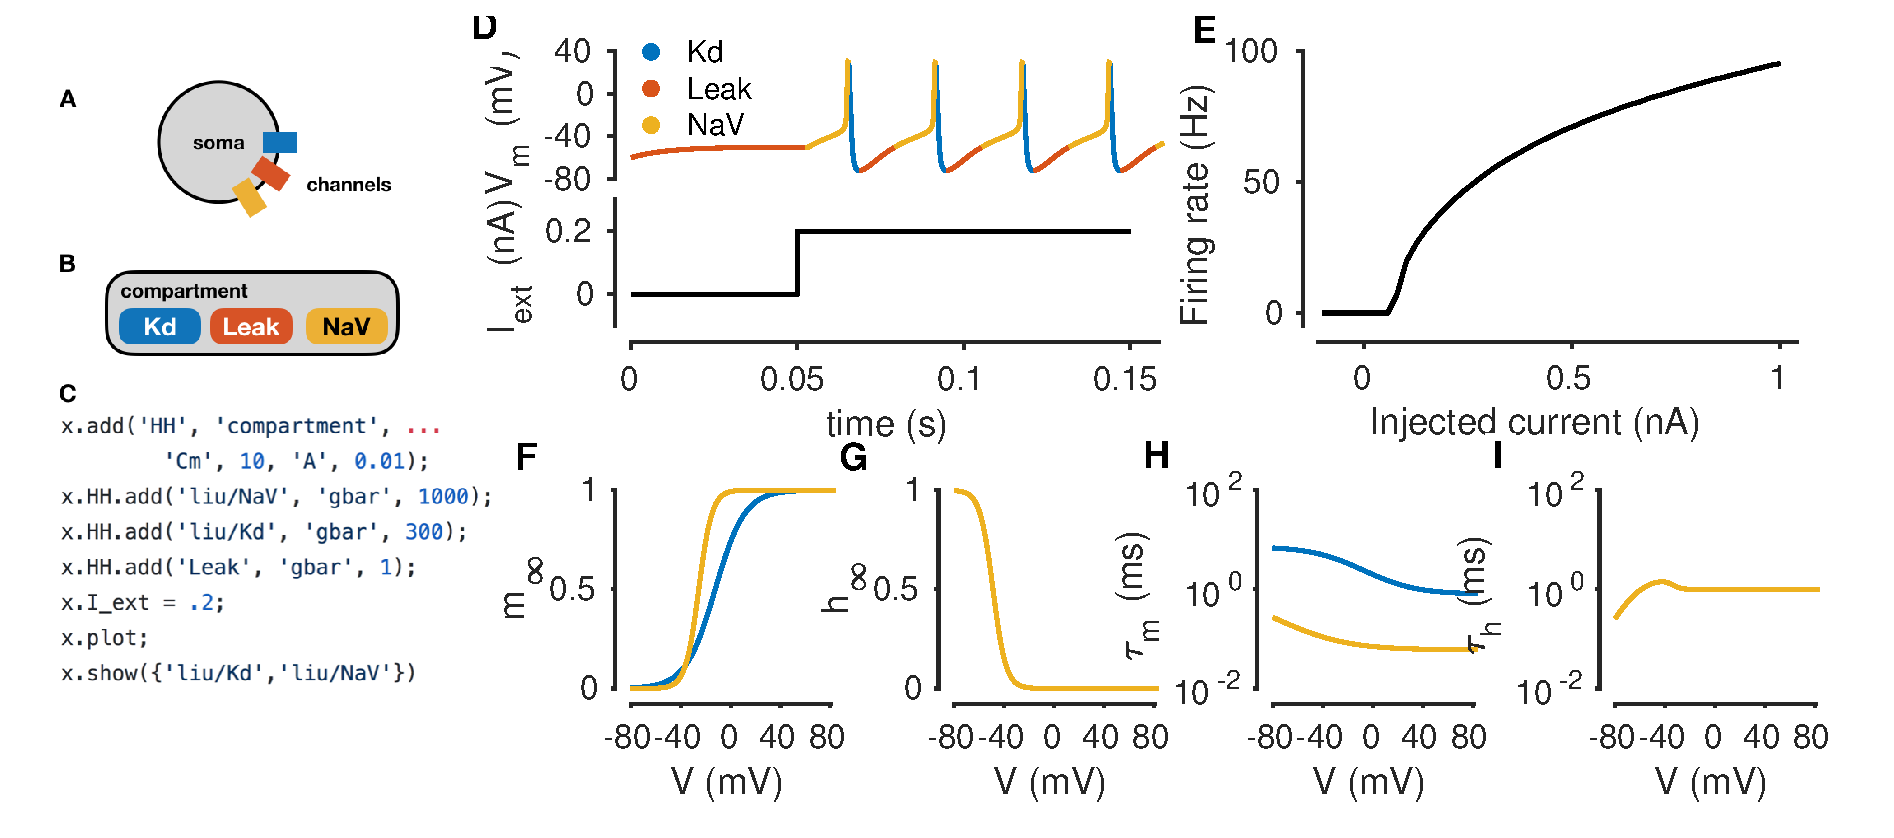
\includegraphics[width=1.0\linewidth]{gfx/figure_HH}
	\caption{Setting up a single-compartment model and injecting current into it. (A) Schematic representation of a single-compartment neuron with three populations of ion channels (colored rectangles). (B) In the simulator, the soma is represented using an object of class $compartment$ and the populations of ion channels are represented by $conductance$ objects contained within the compartment object. (C) The code snippet shown sets up this neuron model, injects current, integrates and plots the voltage, and displays activation functions, all in a few lines of code. (D) Simulated voltage trace of a Hodgkin-Huxley model with three conductances and 0.2 nA of injected current. Colors indicate the dominant current (gold is fast sodium (NaV), blue is delayed rectifier (Kd), red is Leak). (E) firing rate $vs$. current (f-I) curve of this neuron. (F-G) Steady-state gating functions for activation (m) and inactivation (h) gating variables. (H-I) Voltage-dependence of time constants for activation (m) and inactivation (h) gating variables}
	\label{fig:figurehh}
\end{figure}

\begin{figure}[!htb]
	\centering
	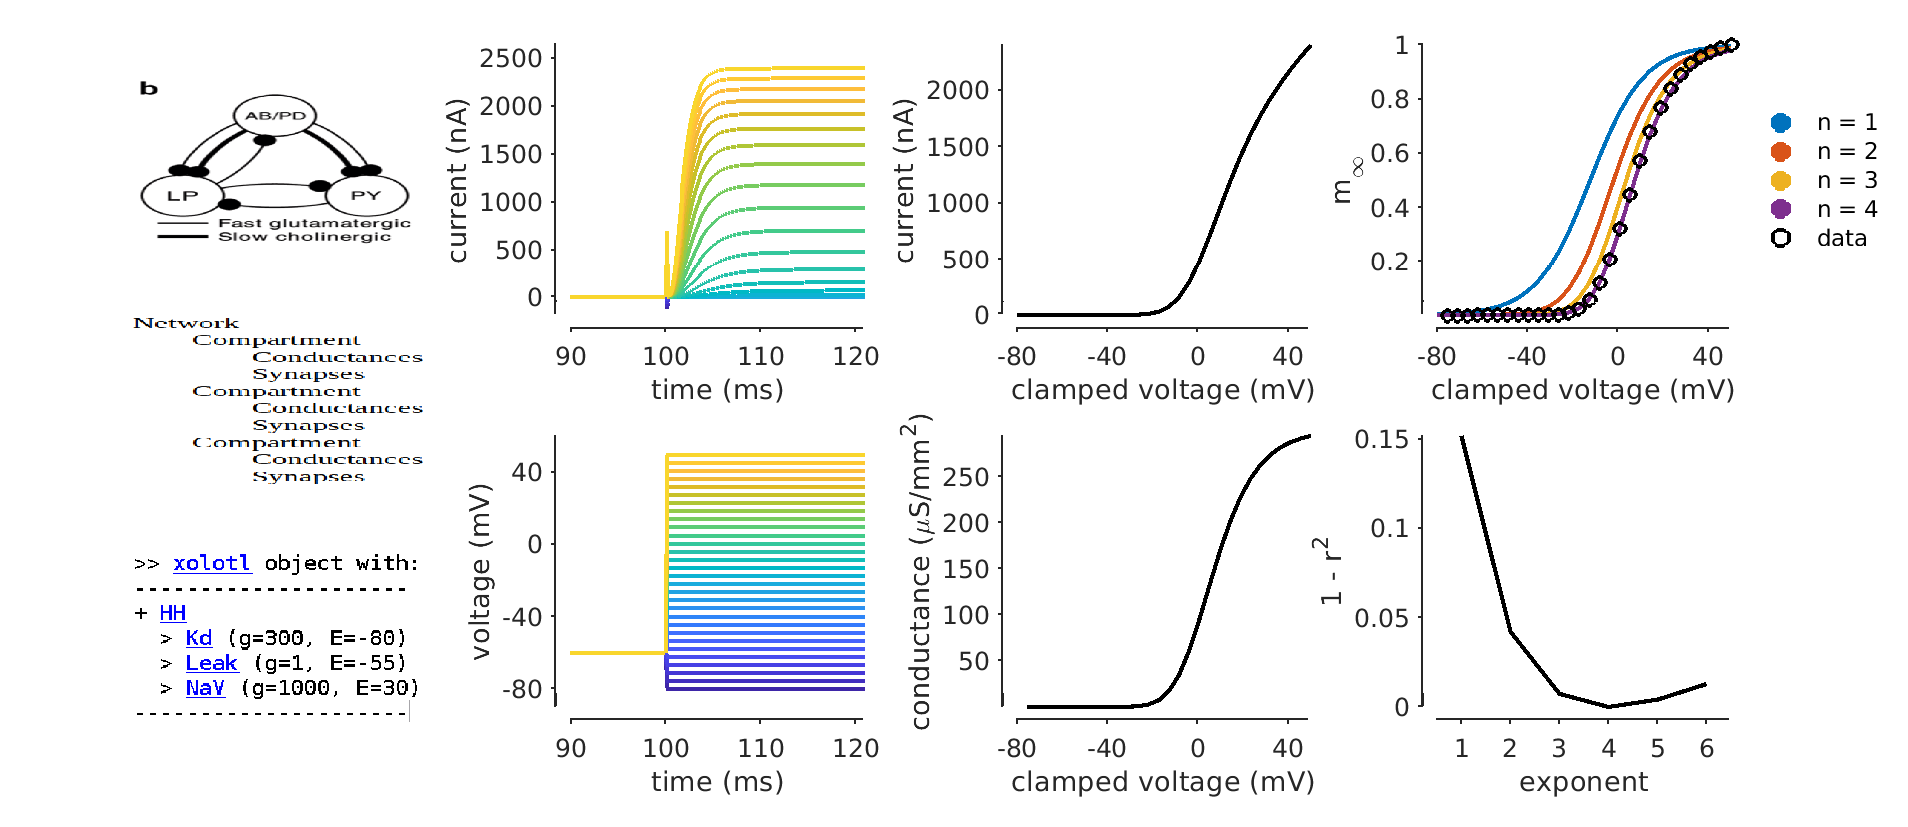
\includegraphics[width=1.0\linewidth]{gfx/figure_clamp}
	\caption{Simulating a voltage-clamp experiment. (A) The diagram shows a cell with delayed rectifier potassium conductance (from \cite{liuModelNeuronActivitydependent1998}) that is being recorded from in two-electrode voltage clamp. (B) The code snippet shown here sets up a model with a single compartment and a single channel type, and clamps the cell to a constant voltage and integrates it. (C) Voltage steps that the cell is clamped to. (D) Current injected into the cell required to clamp it to the voltages in (C). (E) Asymptotic clamped current $vs.$ clamped voltage for this cell. (F) Accounting for the reversal potential of Potassium ions yields the conductance-voltage curve of this channel type. (G) Normalized conductance-voltage curves, with sigmoid fits with various exponents. (H) An exponent of $n=4$ yields the best fit, allowing for the characterization of the activation function of this channel type. }
	\label{fig:figureclamp}
\end{figure}


\begin{figure}[!htb]
	\centering
	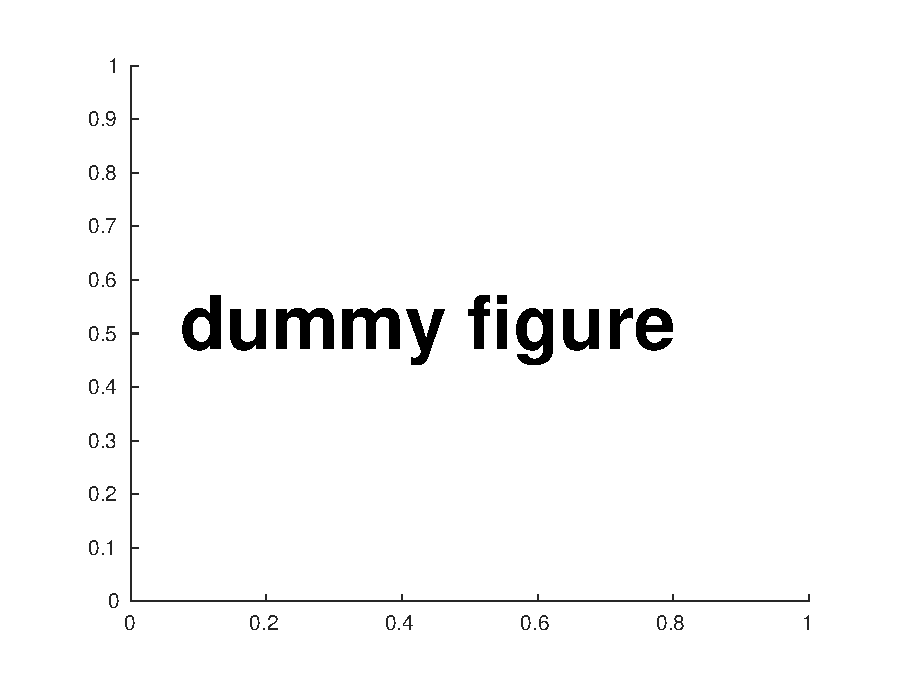
\includegraphics[width=1.0\linewidth]{gfx/figure_mechanism}
	\caption{Modeling intracellular mechanisms. (A) A single-compartment neuron model with 8 channel types. Since there is no mechanism for changing intracellular Calcium in this model, the Calcium level stays constant (B), and the cell tonically spikes (C). Intracellular Calcium buffering and influx through voltage gated Calcium channels (VGCCs) can be modeled using a simple differential equation (D). Code snippet shows how this mechanism can be added to the neuron model (E). The cell now bursts periodically, with synchronized oscillations in intracellular Calcium (F-G). (H) Schematic of Calcium-dependent integral control homeostasis (cite O'Leary et al.). In this feedback system, the rates of mRNA synthesis depend on the Calcium level in the cell, which depends on the membrane voltage, which in turn depends on the conductance density of all channel types, which, through translation, is a function of the mRNA abundance. (I) The code snippet shows how these integral controllers are implemented as \texttt{mechanism} objects, and can be added to conductances. (J) On integrating the model, intracellular calcium levels rise and approach the target (red dashed line). This is accompanied by an increase in the conductance densities of all channels being controlled by this homeostatic mechanism (K). The voltage behavior of the cell changes from silence to bursting with truncated spikes to regular bursting.}
	\label{fig:figuremechanism}
\end{figure}



\begin{figure}[!htb]
	\centering
	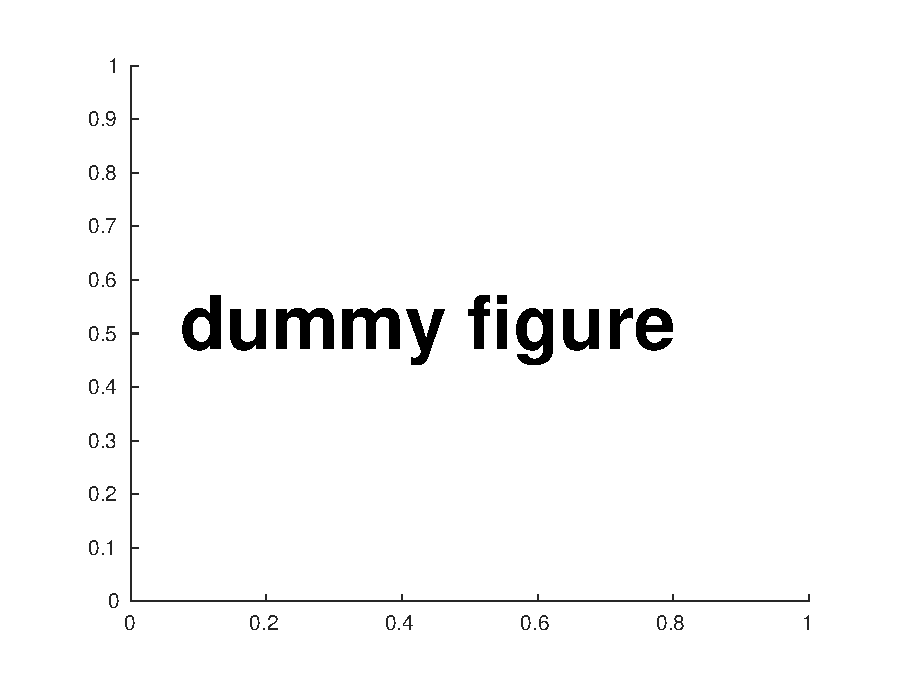
\includegraphics[width=1.0\linewidth]{gfx/figure_snapshot}
	\caption{Snapshots allow the user to bookmark points in parameter and state space of the model and return to them $ad$   $arbitrium$. The initial state (orange disc) of the single compartment model in the previous example is saved using the \texttt{snapshot} method. This method saves all parameters and dynamic variables of the model in a named state. The first column shows the profile of conductances and the voltage dynamics of the model at this point in time. The maximal conductances of the Calcium channels are set to zero (purple), changing the voltage dynamics of the neuron (purple plots). After evolving the model for some time (green), the conductance profile and voltage dynamics returns to a state similar to the initial state (green plots). This configuration is now saved in a state called $final$ and the initial configuration is returned to using the \texttt{reset} method (backwards arrow from green to orange). Another parameter is changed (the Calcium target), and the model is integrated to reach a new state (blue disc) where the voltage dynamics are different from the $initial$ state. In summary, any state can be bookmarked using a descriptive name using the \texttt{snapshot} method, and can be returned to using the \texttt{reset} method.}
	\label{fig:figuresnapshot}
\end{figure}


\begin{figure}[!htb]
	\centering
	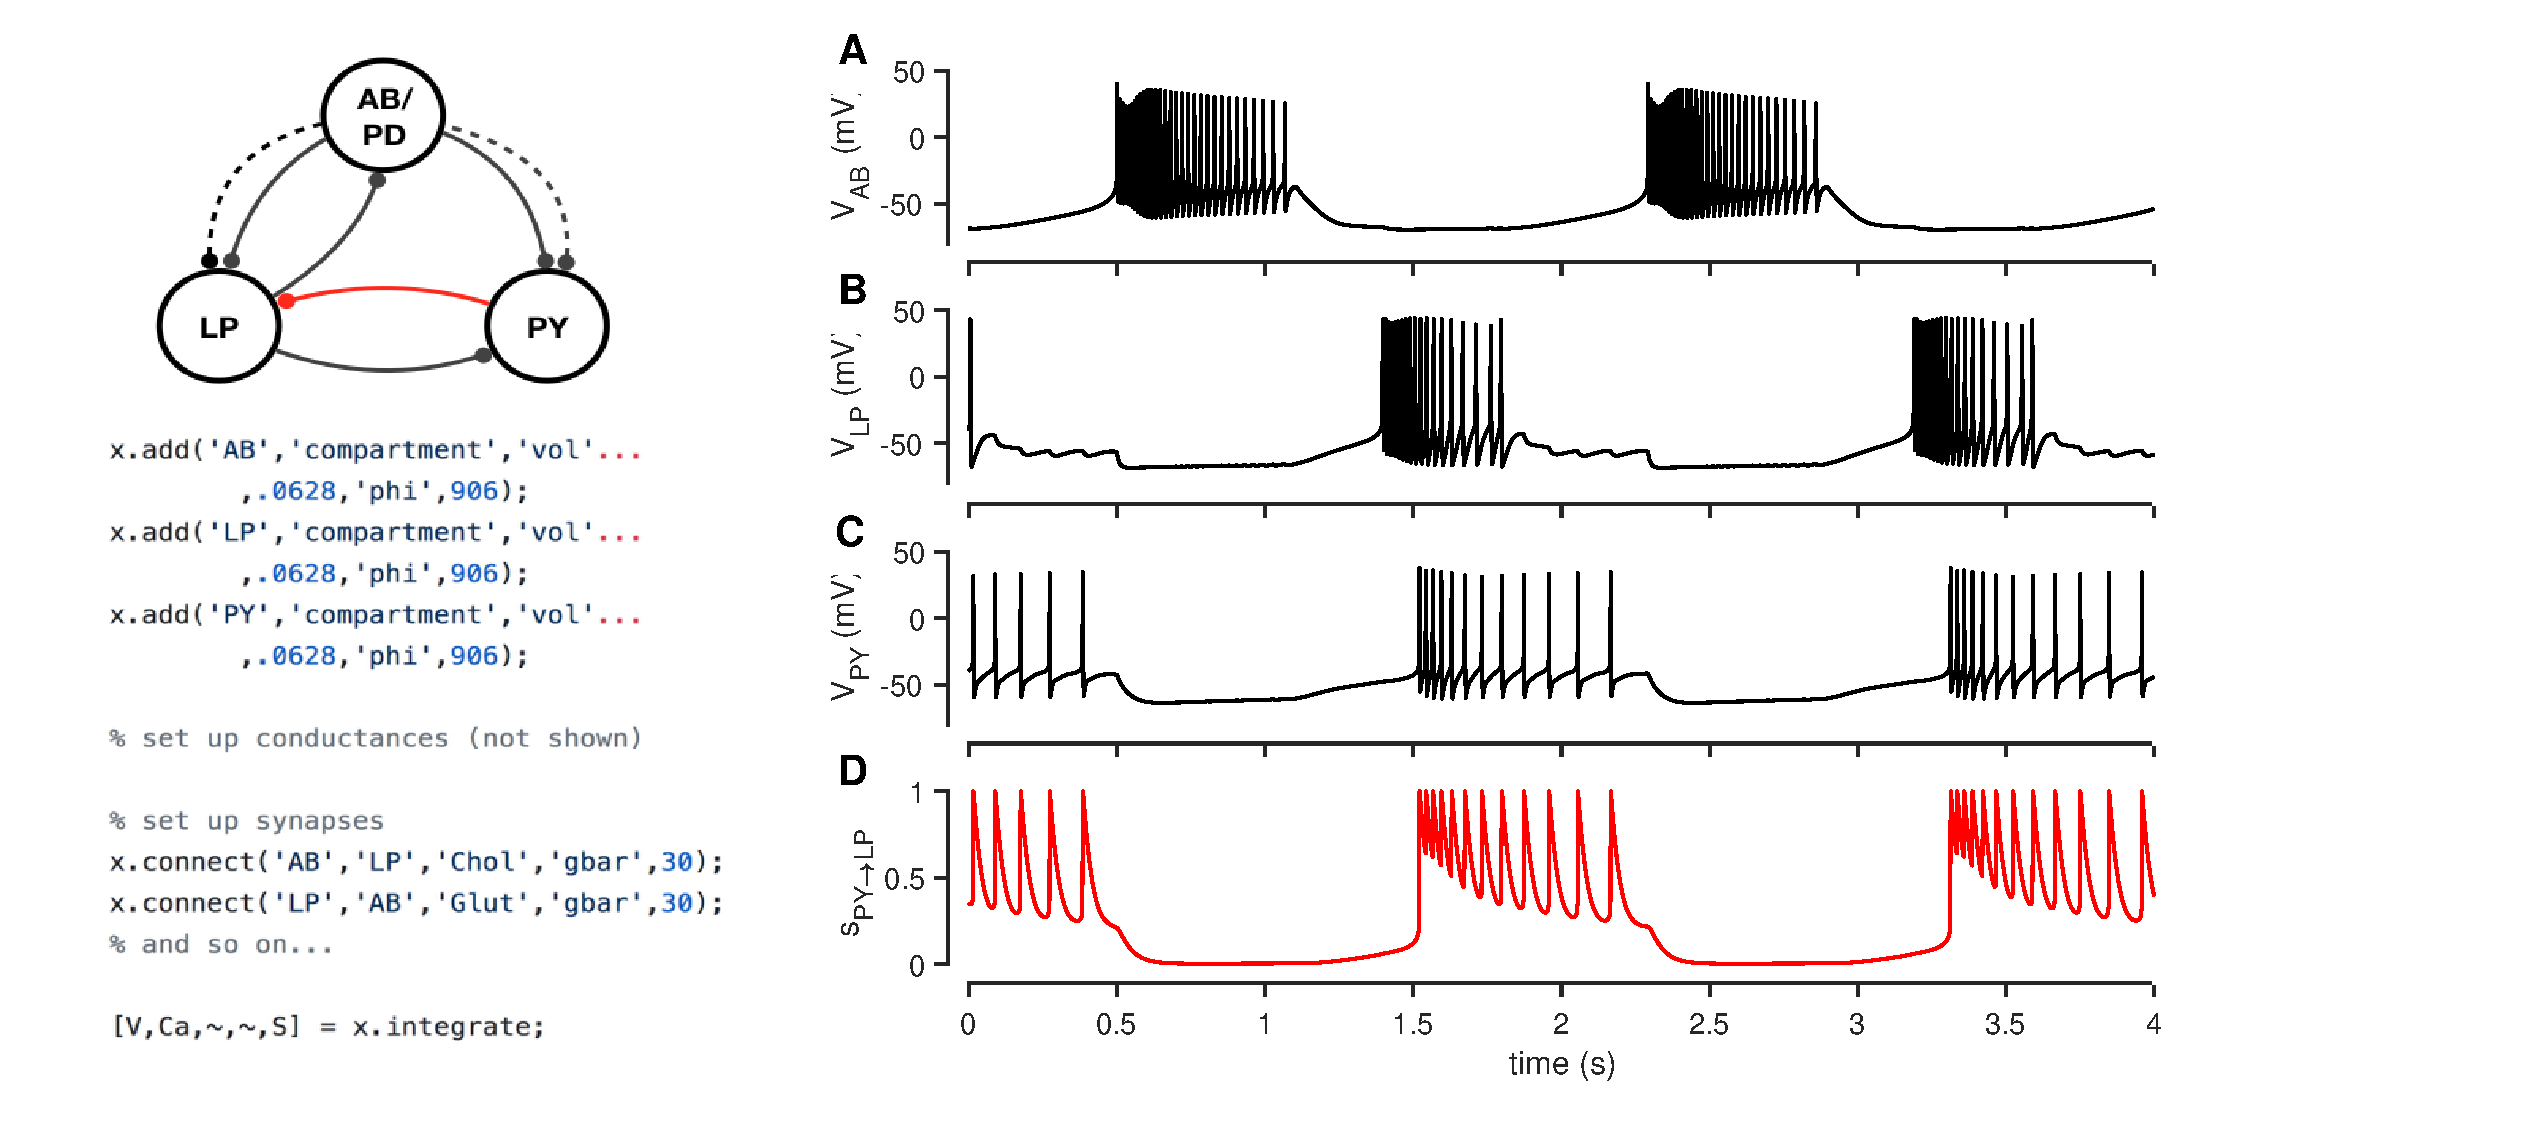
\includegraphics[width=1.0\linewidth]{gfx/figure_network}
	\caption{Simulating a network of conductance-based model neurons. (A) A three-compartment model of the pyloric network in the crustacean stomatogastric ganglion (\cite{prinzSimilarNetworkActivity2004}). Each neuron is modeled with a single compartment with 7-8 intrinsic conductances and 1-3 post-synaptic conductances. Synapses can be one of two types (Cholinergic (dashed lines) or Glutamatergic (solid lines)) and have different kinetics. (B) The code snippet shows how neurons can be created, wired together using synapses, and how the model can be integrated to return voltages and intracellular calcium levels in every compartment, and the state of every synapse. (C-E) Simulated voltage trace of a model network for the three compartments obtained from this simulation. (F) Time series activation variable of the Glutamatergic synapse between PY and LP (red connection in diagram) shows how the synapse becomes active every time the PY neuron spikes.}
	\label{fig:figurenetwork}
\end{figure}



\clearpage

\begin{figure}
	\centering
	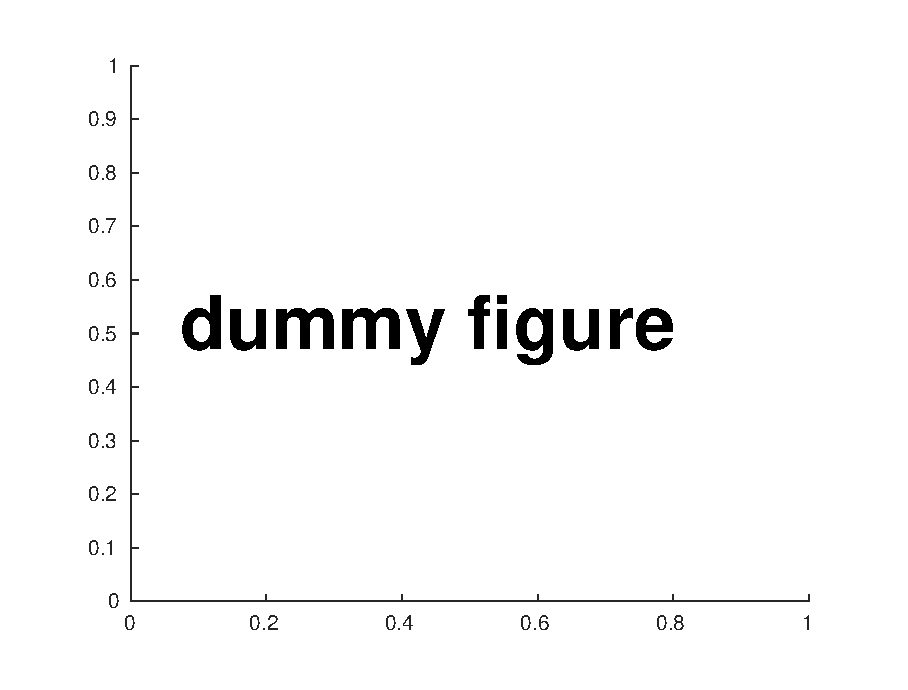
\includegraphics[width=1.0\linewidth]{gfx/figure_manipulate}
	\caption{Manipulating neuron parameters in real time. Any set of parameter in the model can be manipulated; here, the maximal conductance of every conductance type in the model from Figure 1 is being manipulated using the code snippet shown here. The screenshot shows a GUI with sliders for every parameter of interest that is created by the \texttt{manipulate} method, and linked to an arbitrary number of visualization functions. In this example, two visualization functions are used: the built in \texttt{plot} method (A) and a custom function that computes the firing-rate-$vs$.-injected current curve for this neuron (B). Both plots refresh themselves with every movement of any slider, allowing the user to build intuition about how every parameter controls the dynamical behavior of the model. A screen recording of this model being manipulated in real time is included in Supplementary Material XX. }
	\label{fig:figuremanipulate}
\end{figure}

\clearpage

\begin{figure}
	\centering
	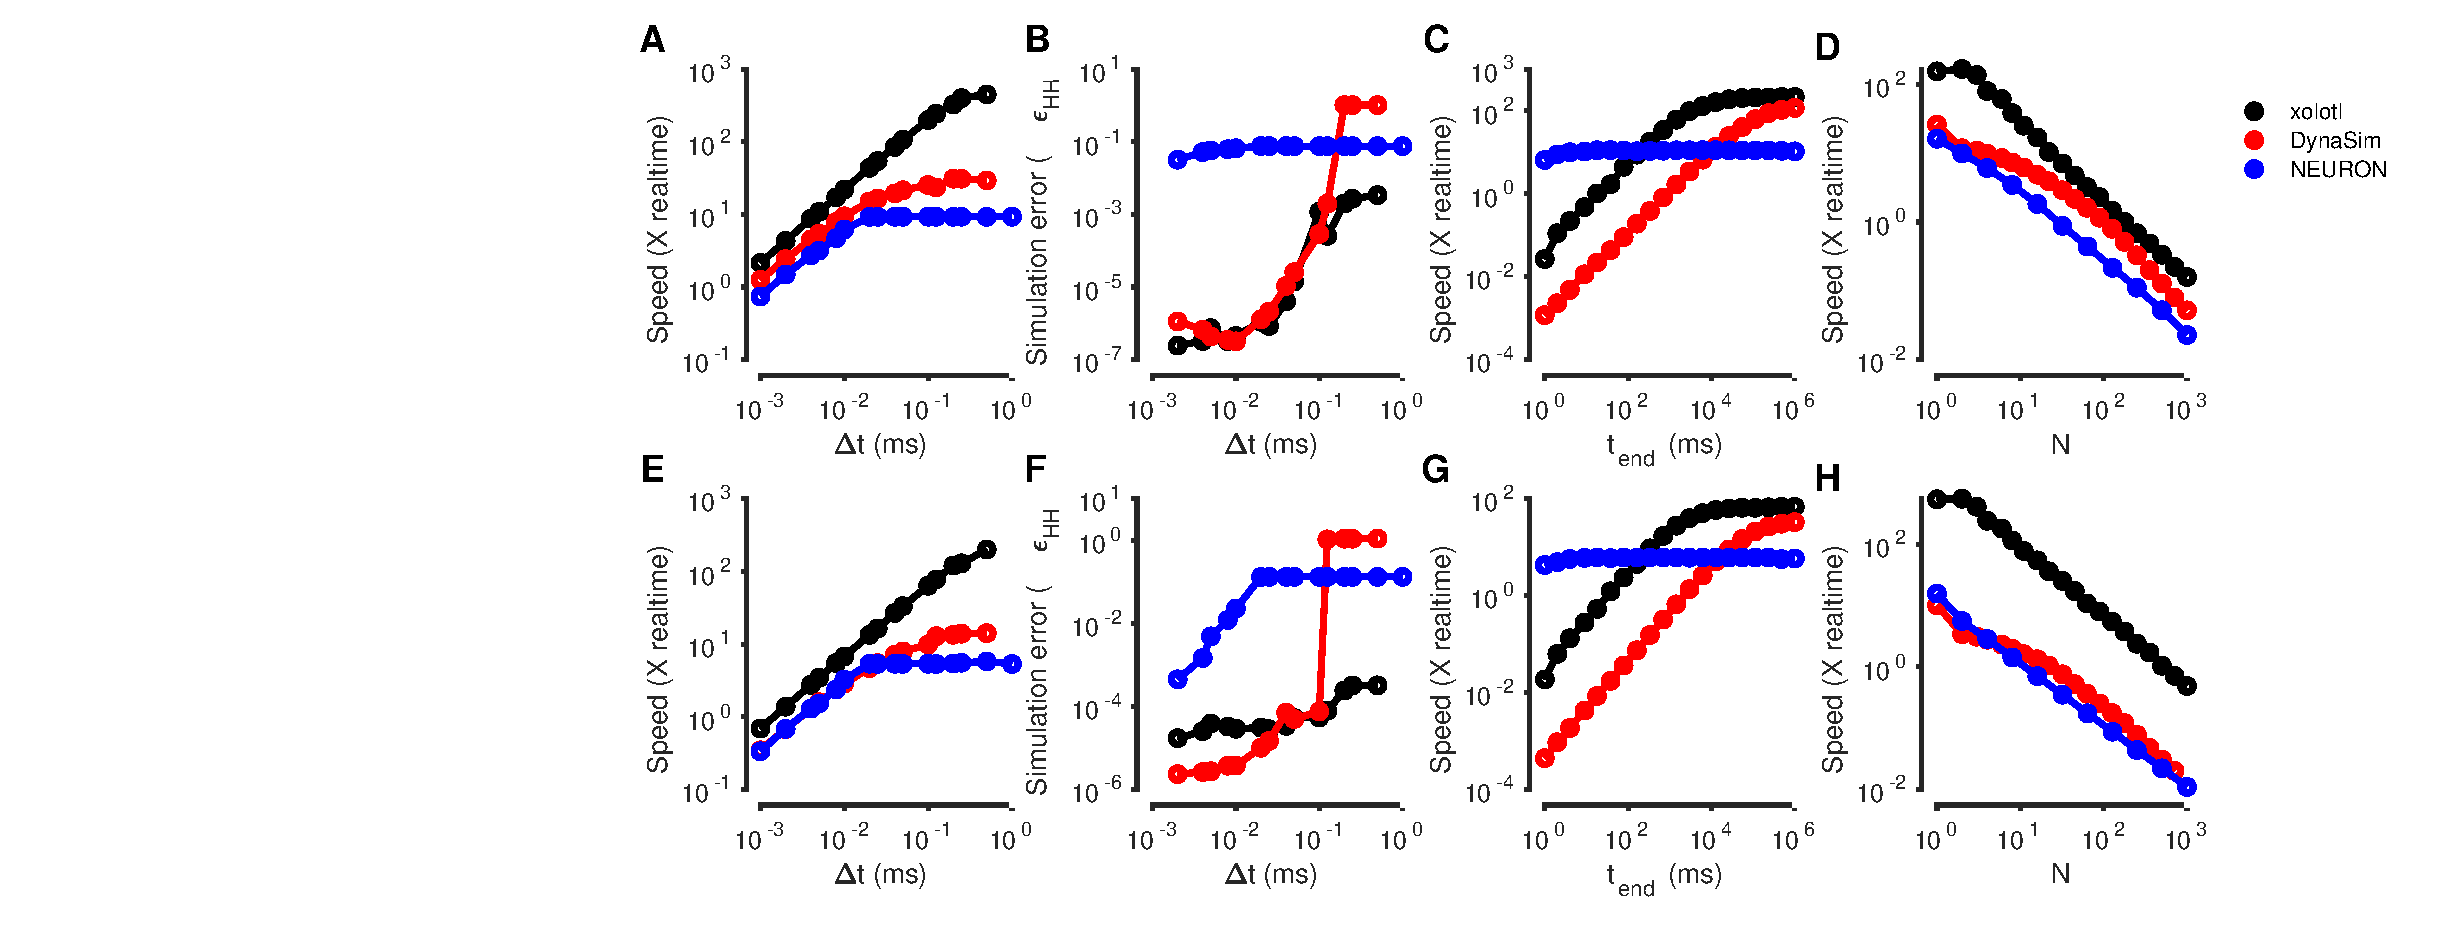
\includegraphics[width=1.0\linewidth]{gfx/figure_benchmark}
	\caption{\texttt{xolotl} benchmarked against \texttt{DynaSim} and \texttt{NEURON}. The top row benchmarks using a tonically-firing Hodgkin-Huxley model with 3 conductances with constant injected current. The bottom row repeats the same benchmarks using a bursting stomatogastric ganglion model with 8 conductances. (A,E) Ratio of run-time to simulation time (speed factor) over increasing integration time step. (B,F) Error over increasing integration time step as computed by the LeMasson matrix where the baseline condition is the voltage trace at $\Delta t = 0.001$ ms. (C,G) Simulations over increasing simulation time where $\Delta t = 0.1$ ms. (D,H) Simulations over increasing number of unconnected compartments.}
	\label{fig:figurebenchmark}
\end{figure}


\end{document}